\Chapter{Koncepció}

%a játékban a csapatok fix létszámmal rendelkeznek viszont bármilyen és bármennyi megjelenhet egy adott osztályokból. ezekkel kapcsolatos harci tevékenységek átgondolása.
%minden tevékenységet ábrákkal szemléltetni

%pálya kialakítása: szakaszok láncolata, pályaszakaszok mérete, hogyan lehet egyikből másikba menni, egymást hogyan követik a pályaszakaszok
%terület meghatározása szakaszra bontás

%az események milyen szinkronban történnek az idő függvényében

%inventory ábrázolása

\Section{A szimulációs környezet bemutatása}

A szimuláció elindítását követően  szembetaláljuk magunkat egy 2D-s oldalnézetes környezettel ahol 8 karakter van és 2 csapat áll egymással szemben. A piros illetve a kék csapat.Mindkét csapatban 4 egyedi karakter lehet.A szimuláció kezdetekor az idő meg van állítva, hogy játékosunk eltudja dönteni melyik karakterrel akar játszani.Az éppen kiválasztott karaktert a felette lebegő nyíl jelzi amelyet a játékos a jobbra-balra nyilakkal tud navigálni a karakterek között,karakterét Enter gombbal tudja kiválasztani és ezután a játék megkezdődik.Minden karakter ami nem került kiválasztásra ágens lesz.A két csapat egymásnak esik.Az ábrán ez megtekinthető:(\ref{fig:scene}.ábra)
\newline
A játék célja az, hogy az egyik csapatnak fel kell vennie az ellenséges csapat zászlóját ezzel megnyerve a játékot.


\begin{figure}[!ht]
	\centering
	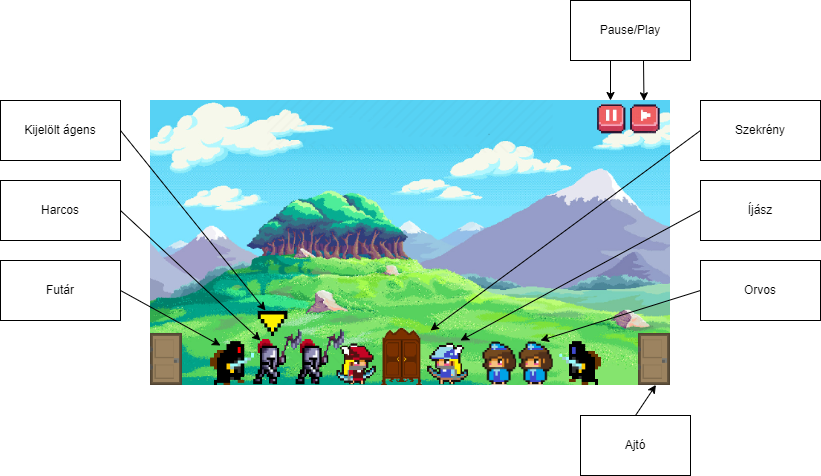
\includegraphics[width=\textwidth]{images/scene.png}
    \caption{környezet}
    \label{fig:scene}
\end{figure}

\Section{Karakterek}

Négy fajta karaktertipus van:
\begin{itemize}
\item Harcos
\item Ijász
\item Orvos
\item Futár
\end{itemize}

Minden karakter tudja végezni a tevékenységüket mozgás közben.
Minden karaktertípus előfordulhat többször is.
Egy csapat létszáma mindig fix 4 fő lehet.

\newpage

\subsection{Karakter tulajdonságok}

Életerő:

\begin{itemize}
\item Minden karakternek van kezdeti életereje aminek értéke a karaktertől függ, tipusa pozitív egész amely 0 érték alá nem mehet.
\item Ha valamelyik karakter életereje eléri a 0 értéket akkor az a karakter meghal.
\item Az életerő csak akkor változik ha karakterünket megsebzik vagy gyógyítják.
\end{itemize}

Védelem:

\begin{itemize}
\item Minden karakternek van egy kezdeti védelme aminek értéke karaktertől függ, típusa pozitív egész.
\item Ha a karakter sebződne ezt az értéket vonjuk le először a támadásból majd a megmaradt sebzéspontokat elszenvedi a karakter.
\end{itemize}

\newpage

Gyorsaság:

\begin{itemize}
  \item Minden karakternek van egy kezdeti gyorsasága aminek értéke karaktertől függ, típusa pozitív egész.
  \item A gyorsaság befolyásolja a karakter mozgási sebességét egyenesen arányosan illetve az akciók visszatöltési képességét fordítottan arányosan.
\end{itemize}

Erő:

\begin{itemize}
  \item Ez a tulajdonság a Harcos osztály egyedi tulajdonsága.Típusa pozitív egész.
  \item Fix értékkel megnöveli támadóértékét illetve a Kivédés \%-os értékét.
\end{itemize}

Ügyesség:

\begin{itemize}
  \item Ez a tulajdonság az Ijász osztály egyedi tulajdonsága.Típusa pozitív egész.
  \item Fix értékkel megnöveli támadóértékét illetve a Kitérés \%-os értékét.
\end{itemize}

Intelligencia:

\begin{itemize}
  \item Ez a tulajdonság az Orvos osztály egyedi tulajdonsága.Típusa pozitív egész.
  \item Fix értékkel megnöveli a Gyógyítás értékét.
\end{itemize}

\begin{table}[!ht]
\centering
\caption{Kezdeti statisztikák}
\label{tab:table1}
\begin{tabular}{|l|c|c|c|c|}
\hline
 & Harcos & Ijász & Orvos & Futár \\
\hline
Erő & 1 & 0 & 0 & 0  \\
\hline
Intelligencia & 0 & 0 & 1 & 0  \\
\hline
Ügyesség & 0 & 1 & 0 & 0 \\
\hline
Életerő & 5 & 5 & 5 & 3 \\
\hline
Védelem & 1 & 1 & 1 & 1  \\
\hline
Gyorsaság & 1 & 1 & 1 &1 \\
\hline
\end{tabular}
\end{table}

\newpage

\subsection{Harcos}

A Harcos egység csak egy egység közvetlen közelében tud támadni vízszintes irányba.
\newline
Csak közelharci fegyvereket használhatnak.

\subsection{Ijász}

Az Ijász egység csak adott távolságon kívül képes támadni fixált vízszintes és függőleges irányba.
Csak távharci fegyvereket képesek használni.

\subsection{Orvos}

Az Orvos egység csak szövetséges karakterek közvetlen közelében gyógyít.
Ha egy karakter meghalt az Orvos nem tudja tovább gyógyítani.
Orvos másodpercenként automatikusan gyógyítja saját magát 1 életerőponttal.
Nem képes fegyvereket használni.

\subsection{Futár}

Feladata, hogy biztosítja a fogyóeszközöket a szövetségesek számára.
Ez az egység csak szövetségeseknek adhat tárgyakat.
Nem képes fegyvereket használni.

\Section{Harc}

\subsection{Harc fázis}

A harc az egy külön fázis, amely akkor kezdődik amikor a csapat minden tagja észleli az ellenfél csapatát és szövetségeseit.A harci fázisnak akkor van vége hogyha az egymással szembenálló valamelyik csapatból az összes tag meghal. A fázis elején dől el, hogy a karakterek kikre tekintenek szövetségesként és kikre ellenfélként.

\subsection{Sebzés kalkulálása}

Sikeres támadás esetén a sebzés mértéke 0 ha a harci hatások valamelyike érvényesül vagy időben lett használva a gugolás.Más esetben a sebzés mértékét befolyásolja az adott karakter védelme, ez az érték levonódik a sebzés értékéből majd az eredményt levonjuk a védekező karakter életerejéből.

\newpage

\subsubsection{Harci hatások}

Kitérés:
\begin{itemize}
\item Ez a hatás \%-os eséllyel aktiválódik minden egyes ellenfél által bevitt sikeres közelharci támadás esetén.
\item Ez az esély egyenesen arányosan függ a karakter státuszaitól.
\item Ez egy állandó hatás.Csak az Ijász rendelkezik ezzel a hatással.
\end{itemize}

Védekezés:
\begin{itemize}
\item Ez a hatás \%-os eséllyel aktiválódik minden egyes ellenfél által bevitt sikeres támadás esetén.
\item Ez az esély függ a pajzs fejlettségétől,karaterünk státuszától.
\item Ez egy állandó hatás.Csak a Harcos rendelkezik ezzel a hatással.
\end{itemize}

\Section{Szint}

Minden legyőzött ellenfél után a karakter kap tapasztalai pontot attól függően, hogy melyik karakter osztályát ölte meg.
Minden szintlépés után a karakter kap egy státuszpontot amit elhasználhat valamelyik statisztika növelésére.

\begin{table}[!ht]
\centering
\caption{Szintezés}
\label{tab:table2}
\begin{tabular}{|l|c|c|c|c|}
\hline
 & Harcos & Ijász & Orvos & Futár \\
\hline
Tapasztalati pont & 3 & 5 & 2 & 1   \\
\hline
Szintlépés tapasztalati pont alapján & 5 & 5 & 5 & 5  \\
\hline
Statisztikák növelése & +1 & +1 & +2 & +3 \\
\hline
Maximum pont egy statisztikára & 10 & 10 & 10 & 10  \\
\hline
\end{tabular}
\end{table}

\subsection{Pontok elosztásának prioritása}

Az ágenseknél egy megadott prioritás alapján dől el, hogyan osztódnak el a pontok.

\begin{table}[!ht]
\centering
\caption{Prioritás}
\label{tab:table3}
\begin{tabular}{|l|c|c|c|c|}
\hline
 & 1. & 2. & 3. & 4. \\
\hline
Harcos & Erő & Védelem & Életerő & Gyorsaság   \\
\hline
Ijász & Ügyesség & Életerő & Gyorsaság & Védelem  \\
\hline
Orvos & Intelligencia & Gyorsaság & Védelem & Életerő \\
\hline
Futár & Gyorsaság & Életerő & Védelem &  \\
\hline
\end{tabular}
\end{table}

\newpage

\Section{Tárgyak}

\begin{table}[!ht]
\centering
\caption{Tárgyak}
\label{tab:table4}
\begin{tabular}{|l|c|c|c|c|}
\hline
 & Osztály &Típus & Támadás & Védelem  \\
\hline
Kard & Harcos & Közelharc & 1-5 & 0 \\
\hline
Íj & Ijász & Távharc & 1-5 & 0  \\
\hline
Mellvért & Harcos & Közelharc & 0 & 3   \\
\hline
Mellény & Ijász & Közelharc & 0 & 1   \\
\hline
Köpeny & Orvos & Közelharc & 0 & 2    \\
\hline
Ruha & Futár & Közelharc & 0 & 2    \\
\hline
Lábvért & Harcos & Közelharc & 0 & 3    \\
\hline
Vászonnadrág & Ijász & Közelharc & 0 & 1    \\
\hline
Orvosi nadrág  & Orvos & Közelharc & 0 & 2    \\
\hline
Nadrág & Futár & Közelharc & 0 & 2   \\
\hline
\end{tabular}
\end{table}

Speciális tárgyak:
\begin{itemize}
  \item Kötszer:Csak az orvos képes használni.Fogyóeszköz. 3 életerőt lehet vele gyógyítani.
  \item Nyílvessző:Csak Ijász képes használni.Fogyóeszköz.Ha elfogy az egység nem tud támadni.
  \item Pajzs:Csak a Harcos használhatja. 10\% védekezési esélyt nyűjt de csak közelharcban.
\end{itemize}

\Section{Hátizsák}

\begin{itemize}
  \item A hátizsák egy megjelenő menü amit a TAB billentyűvel lehet megnyitni,1 küldetés,2 páncél,1 fegyver,10 tárolóhelyből áll.
  \item Teljesen megegyező és különböző tárgyak külön-külön helyen fognak tárolódni.
  \item A karakterek közötti tárgy átadásnál a tárgy az adó karakter leltárából törlődik a vevő karakternél megjelenik.
  \item Ha egy tárgyat kihúzunk a hátizsák menüjén kívülre, akkor a tárgy törlődik.
  \item Más szövetséges karakterek hátizsákját csak a Futár osztály láthatja olyan karakterenk nem látja akiket ellenségként észlel.
  \item Ha egy karakter meghal a teljes hátizsákja törlődik.
  \item A küldetés tárolóhelyre csak a zászló kerülhet.
\end{itemize}

\subsection{Osztályok leltára}
\begin{itemize}
  \item Az Ijász osztály teljes leltára a szimuláció kezdetekor  nyílvesszővel van feltöltve.
  \item Az Íjász leltárában csak nyílvesszők lehetnek.
  \item Az Orvos osztály teljes leltára a szimuláció kezdetekor kötszerrel van feltöltve.
  \item Az Orvos leltárában csak kötszerek lehetnek.
  \item A Futár leltára a szimuláció kezdetén félig nyílvesszővel, félig kötszerrel van feltöltve.
  \item Csak a Futár osztály képes karakterek között tárgyakat átadni.
  \item A Harcos osztály leltárja üres.
  
\end{itemize}

\Section{Harcon kívüli tevékenységek}

Harcon kívül a karakterek egy megadott sorrendben egymás háta mögött mennek követve a sorban elölálló karaktert.A sorrend előlről hátrafelé a következő:
\begin{itemize}
\item Harcos
\item Ijász
\item Orvos
\item Futár
\end{itemize}
Ha egy osztály-ból több is előfordul akkor kettejük között a sorrend véletlenszerűen dől el.

\subsection{Általános akciók}

Ezek akciók csak 1 dimenziósak és csak az x tengellyel párhuzamos síkokon érvényesülnek.

Mozgás akció:

\begin{itemize}
  \item Minden karakter alkalmazza.
  \item A karakter egy fix távolságot tesz meg vagy jobbra vagy balra.
  \item A játékos Jobbra az A  balra a D billentyűvel tud menni.
  \item Ez az akció harc fázisban is müködik.
\end{itemize}

Ajtó akció:

\begin{itemize}
  \item Minden karakter egyesével tudja használni az ajtót, hogy egyik területről átmenjenek a másikra.
  \item A játékos az F billentyűvel tudja kinyitni az ajtót.
\end{itemize}


\Section{Harci tevékenységek}

Szövetséges ágensek nem blokkolják egymást a mozgásban de csak harci tevékenységek közben.
\newline
A harc fázisba lépést követően minden karakter egyedi tevékenységeket fog különböző feltételek alapján elvégezni.
\newline
Ezek akciók csak 1 dimenziósak és csak az x tengellyel párhuzamos síkokon érvényesülnek.

Támadás akció:

\begin{itemize}
\item Ezt a képességet használó karakter csökkenteni tudja más karakterek életerejét.
\item Ha egy karakter életereje 0 akkor nem lehet tovább támadni.
\item Ezt az akciót csak időközönként lehet használni.Karakterfüggő, hogy mekkora visszatöltési ideje van ennek az akciónak.
\item A játékos a SPACE billentyűvel támadhat.
\end{itemize}

Gyógyítás akció:

\begin{itemize}
  \item Ezt a képességet használó karakter vissza tudja tölteni más karakterek életerejét.
  \item Maximum életerő vagy 0 életerő esetén nem lehet gyógyítani.
  \item A játékos az E billentyűvel tud gyógyítani.
\end{itemize}

Gugolás akció:

\begin{itemize}
  \item Az ágensek esetében van \%-os esély arra, hogy gugolás akciót használjon , abban a pillanatban amikor egy Ijász éppen támad ezzel elkerülve a sebzést.
  \item A gugolás hatása csak távharci támadás esetében érvényesül.
  \item A játékos a C billentyűvel tud gugolni.
\end{itemize}

Átadás akció:

\begin{itemize}
  \item Ezt a képességet használó karakter tárgyakat tud átadni más karaktereknek.
  \item A játékos az F billentyűvel tud átadni tárgyakat.
\end{itemize}

\subsection{A harcos tevékenységei}
\begin{itemize}
  \item Megvizsgálja hogy a közvetlen közelében van-e ellenség ha nincs akkor addig megy amíg nem lesz a közelében ellenfél.
  \item Ha hatótávolságba ér akkor támad a támadást addig végzi amíg az adott ellenfél meg nem hal vagy nem kezd el kimenni a támadás hatósugarából.
  \item Harcosok közelharci támadás hatóköréből nem tudnak menekülni viszont minden közelharci támadásra van esélyük a kivédésre.
  \item Ha az ellensége akivel harcol meghal elindul a következő legközelebbi ellenség irányába és megtámadja.
\end{itemize} 

\subsection{Az Ijász tevékenységei}

\begin{itemize}
  \item Az Ijásznak a harc kezdetekor el kell döntenie, hogy az ellenség csapatából kit fog támadni, csak azokat az ellenfeleket képes támadni akik a hatótávjában vannak prioritás alapján.
  \item Eldöntés után addig támadja ezt a karakter amíg az meg nem hal vagy ki nem fogy a Nyílvesszőkből.
  \item Ha meghal a karakter akit támadott akkor a prioritásban következő ellenséget támadja.
  \item Minden egyes támadás után az Ijász leltárából eltünik egy nyilvessző.
  \item Ha az Ijász karakternek elfogy a leltárából a nyílvessző akkor üzen a Futár karakternek, hogy szüksége van a számára megfelelő tárgyakra.
  \item Ha elfogyott a nyílvessző és nem kap utánpótlást akkor addig nem támad amíg nem lesz a leltárában nyílvessző.
  \item Ez a karakter mindig tart egy fix távolságot a legközelebbi ellenféltől.
\end{itemize}

Az Ijász támadási prioritása:

\begin{itemize}
  \item Gyógyító
  \item Futár
  \item Ijász
  \item Harcos
\end{itemize}

\subsection{Az Orvos tevékenységei}

\begin{itemize}
  \item Az Orvos folyamatosan a szövetségesei életerejét vizsgálja,ha egy karakter életereje x\% alá esik akkor üzen az Orvos karakternek, hogy gyógyításra van szüksége.
  \item Ennek hatására az Orvos odamegy az üzenet küldő karakter közvetlen közelében és elkezdi őt gyógyítani.
  \item A gyógyítás fix időn belül megtörténik és eltünik egy kötszer az Orvos leltárából.
  \item A prioritás mindig annál a karakternél van aki a legrégebben küldte az üzenetet.
  \item Csak az Orvos osztállyal lehet gyógyítani.
\end{itemize}

\newpage

\subsection{A Futár tevékenységei}

\begin{itemize}
  \item A Futár folyamatosan a szövetséges Orvos illetve Ijász leltárát vizsgálja.
  \item Ha az Orvos illetve a Ijász karakternek elfogy a leltárából a kötszer vagy nyílvessző akkor üzen a Futár karakternek, hogy szüksége van a számára megfelelő tárgyakra.
  \item Erre az üzenetre reagálva a Futár feltölti az üzenetet küldő karakter leltárját azzal a tárggyal amit kért.
  \item Mindkét osztály csak akkor küld üzenetet ha teljesen kifogytak.
  \item A prioritás mindig annál a karakternél van aki a legrégebben küldte az üzenetet.
  \item Futárok egymásközött tudnak átadni tárgyakat.
  \item A harc fázis végén feltőltődik a futár leltára félig nyílvesszővel félig kötszerrel.
  \item Csak a Futár osztállyal lehet tárgyakat átadni.
\end{itemize}

\Section{Az események müködése}

A alábbi akciókat tudják az ágensek egymástól függetlenül végezni:
\begin{itemize}
  \item Mozgás
  \item Ajtó
  \item Támadás
\end{itemize}
Harcon kívüli akciókat nem lehet használni, harc fázisban és fordítva sem.
\begin{itemize}
  \item Gugolás akció közben nem tud semmilyen más tevékenységet végezni csak megszakítani lehet bármivel.
  \item Mozgás akció közben az összes harci tevékenységet lehet végezni.
  \item Támadás akció közben nem lehet semmilyen más tevékenységet végezni csak megszakítani lehet bármivel.
  \item Átadás akció esetében az adó karakter nem tud más tevékenységet végezni, viszont a vevő karakternek csak mozogni nem szabad az akció befejezéséig különben megszakítja az átadást.
  \item Gyógyítás esetében az akciót végző karakter nem tud más tevékenységet végezni de a gyógyított karakternek csak mozogni nem szabad az akció végéig különben megszakítja a gyógyítást.
  \item Ajtó akció közben nem lehet más tevékenységet végezni és megszakítani sem lehet.
  \item A harci hatások minden tevékenység közben aktívak ha rájuk vonatkozó feltételek teljesülnek.
\end{itemize}


\Section{Hogyan észleli az ágens az őt körülvevő környezetet}

\begin{itemize}
  \item A szövetséges és ellenséges karaktereket kinézet alapján különbözteti meg.
  \item A zászló észlelésének kivételével mindent egy adott területen képesek érzékelni amit maga a háttér határol be.
  \item Az ágensek nem mozdulnak kezdeti helyükről amik nem észlelnek ellenséget.
  \item Harci fázis után mindig abba az irányba haladnak tovább amerre az ellenséges zászlót érzékelik.
  \item Kinézet alapján dől-el, hogy a zászló szövetségeseké vagy ellenségé.
  \item A zászló helyzetét tudják a szimuláció kezdetétől.
  \item A zászló annak a karakternek a küldetés tárolóhelyére kerül aki a leghamarabb elér hozzá.
\end{itemize}









